\documentclass[a4paper,12pt]{article}
\usepackage[a4paper,margin=0.8in]{geometry} % <-- You can adjust the margin size here
\usepackage{titling}
\usepackage{graphicx}
\usepackage{subcaption}
\usepackage[justification=centering]{caption}
\usepackage{lipsum}

% Package for table of contents formatting
\usepackage{tocloft}
\renewcommand{\cfttoctitlefont}{\large\bfseries} % Format table of contents title

% Other configurations
\usepackage{tabularx} % extra features for tabular environment
\usepackage{amsmath}  % improve math presentation
\usepackage{amsfonts}
\usepackage{amsthm}

% Package for long table
\usepackage{longtable}
\usepackage{multirow}
\usepackage{array}
\usepackage{booktabs}

% Package for algorithm
\usepackage{algorithm}
\usepackage{algpseudocode}

\newtheorem{theorem}{Theorem}
\newtheorem{definition}{Definition}
\newtheorem{lemma}{Lemma}
\newtheorem{problem}{Problem}


\usepackage{cite} % takes care of citations
\usepackage[final]{hyperref} % adds hyper links inside the generated pdf file
\usepackage{enumerate}

\usepackage{titlesec} % Change Title size
\usepackage[numbered,framed]{matlab-prettifier}
\usepackage[T1]{fontenc}

\usepackage{forest} % For drawing directory tree

\usepackage{circuitikz} % Circuit drawing


\hypersetup{
	colorlinks=true,       % false: boxed links; true: colored links
	linkcolor=black,        % color of internal links,
	citecolor=black,
}



% ++++++++++++++++++++++++++Code global config begin++++++++++++++++++++++++++
% Code block universal settings, all lstdefinestyle must appeared below this block!
\usepackage{listings}
% use txtt global font
\usepackage[T1]{fontenc} % Add font options
\DeclareFixedFont{\codefont}{T1}{txtt}{m}{n}{12} % other options: txtt -> cmtt, pcr, fvm, zi4; m -> bx, n; 12 -> (fontsize)

% Define colors
\usepackage{color}
\usepackage{tikz} % colorlet need this
\definecolor{commentgreen}{rgb}{0,0.5,0}
\colorlet{framegray}{black!40}
\definecolor{stringred}{rgb}{0.6,0,0}

% Global config
\lstset{
	backgroundcolor=\color{gray!7},
	numbers = left, % show line number on the left
	numberstyle = \small\color{framegray}, % line number color
	basicstyle = \codefont, % code font
	columns = flexible, % make the spacing between characters compact
	keepspaces = true,  % keeps spaces in text, useful for keeping indentation of code (needs columns=flexible)
	% captionpos = b, % caption at the bottom
	commentstyle = \color{commentgreen}, % comment color
	frame = single, % display frame
	stringstyle = \color{stringred}, % Strings in red
	rulecolor = \color{framegray}, % frame color
	showstringspaces = false, % don't mark spaces in strings
	breaklines = true, % break long lines
	tabsize = 4, % tab size
}
% +++++++++++++++++++++++++++Code global config end+++++++++++++++++++++++++++

% ++++++++++++++++++++++++++Python local config begin++++++++++++++++++++++++++
% Must placed below the global settings
% Custom colors for python only
\definecolor{emphblue}{rgb}{0,0,0.5}
\definecolor{keywordpink}{RGB}{128, 0, 128}
% this will override the global settings
\lstdefinestyle{custompython}{
	language = Python,
	emph = {__init__, self}, % Custom highlighting
	emphstyle = \color{emphblue},  % Highlighted words in deepblue
	keywordstyle = \color{keywordpink},
	upquote = true, % single quotes in straight quote
}
% ++++++++++++++++++++++++++++Python local config end++++++++++++++++++++++++++++

% ++++++++++++++++++++++++++Bash local config begin++++++++++++++++++++++++++
% Must placed below the global settings
% this will override the global settings
\lstdefinestyle{custombash}{
	language = bash,
	basicstyle = \ttfamily, % Monospaced font
	keywordstyle = \color{blue}\bfseries, % Keywords in bold blue
	stringstyle = \color{green}, % Strings in green
	commentstyle = \color{gray}, % Comments in gray
	morekeywords = {sudo, ls, cd, rm, mkdir}, % Add common Bash commands
}
% +++++++++++++++++++++++++++Bash local config end+++++++++++++++++++++++++++






\begin{document}

\begin{center}
    \textbf{ } \\
    \vspace{4em}
    {\huge \textsf{ML Project 2 Report}} \\
    \vspace{1.5em}
    {\large \textsf{CNN for Image Classification}} \\
    \vspace{1em}
    \vspace{1.5cm}
    \textbf{Name:} Jinming Ren \\
    \vspace{0.5em}
    \textbf{UESTC ID:} 2022190908020 \\
    \vspace{0.5em}
    \textbf{UofG ID:} 2840216R \\
    \vspace{0.5em}
    \textbf{Date:} \today \\
    \vspace{0.5em}
    \vspace{0.5cm}
    \textbf{University:} UoG-UESTC Joint School \\
    \vspace{1.5em}
\end{center}

\newpage
\tableofcontents
\listoffigures
\listoftables


\newpage

\section{Introduction and Problem formulation}

Machine learning has become increasingly important in solving image classification tasks, which require efficient and accurate models to identify and categorize images into predefined classes. This project focuses on comparing the performance of a classical machine learning model, the Decision Tree Classifier, with a state-of-the-art deep learning model, AlexNet, for a multi-class waste classification task.

The dataset used for this study is a COCO-style dataset containing annotations for seven distinct waste categories. The objective is to preprocess the dataset, train both models on the training set, evaluate their performance on the test set, and analyze their behavior across various metrics, such as accuracy, precision, recall, and F1-score.

The project involves:
\begin{enumerate}
	\item \textbf{Data Preparation:} Splitting the dataset into training, validation, and testing subsets, followed by preprocessing operations such as cropping, resizing, normalization, and feature extraction (e.g., HOG for the Decision Tree).
	\item \textbf{Model Training:} Implementing AlexNet and Decision Tree Classifier to train on the preprocessed data using different optimization strategies.
	\item \textbf{Performance Evaluation:} Using confusion matrices and classification metrics to compare the models’ ability to classify waste into their respective categories.
\end{enumerate}

This report highlights the strengths and weaknesses of each model and provides insights into the suitability of classical and deep learning approaches for image classification tasks.

\section{Methodology}

\subsection{Data Loading and Processing}

\subsubsection{Training Set Splitting}

The first thing to do is to split the COCO-style dataset into three different categories for different purposes:

\begin{itemize}
	\item \textbf{Training Set:} Used to \textit{train} the model by optimizing the weights based on the loss function.
	\item \textbf{Validation Set:} Evaluates the model \textit{during training} to tune hyperparameters and monitor overfitting.
	\item \textbf{Testing Set:} Provides an evaluation of the model’s performance after training.
\end{itemize}

If one uses the same set, then the model will be biased towards the data it has seen before and will not generalize well to new data. The detailed split procedure is described in Appendix \ref{app:splitting}.

\subsubsection{Image Preprocessing}

Before feeding the images in the dataset into the network, we need to preprocess the images. The following steps are taken:

\begin{itemize}
	\item \textbf{Cropping:} Crop each image in the dataset according to a predefined box. Each image annotation includes a bounding box in the format of \texttt{[x, y, width, height]}. For example, If bbox = \texttt{[50, 30, 100, 150]}, the box starts at pixel (50, 30) and spans 100 pixels wide and 150 pixels tall.
	\item \textbf{Resizing:} Resize the cropped image to a fixed size. The size of the image is set to $192\times192$ pixels in our case.
	\item \textbf{Tensorization:} Convert the image into a tensor, which the neural network can process efficiently.
	\item \textbf{Normalization:} Translate each pixel values in all RGB channels based on a predefined mean value and normalize them within a number in $[0,1]$, i.e.,
	$$
	\text{Normalized Pixel} = \frac{\text{Pixel value} - \text{Mean}}{\text{Standard Deviation}}
	$$
\end{itemize}

This part is accomplished in \texttt{dataset.py} as shown in Appendix \ref{app:dataset_py}. This is only for experiment purposes. In actual training process, the image preprocessing is done together with the network training as shown in Appendix \ref{app:train_py}.

\subsection{Network Implementation}
\label{sec:network_implementation}

AlexNet is used to implement the network. The architecture of AlexNet is shown in Figure~\ref{fig:alexnet}. The detailed architecture and Python realization is shown in Appendix \ref{app:alexnet} and \ref{app:model_py}.

\begin{figure}[h!]
	\centering
	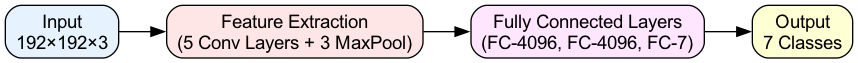
\includegraphics[width=\textwidth]{../image/AlexNetStruct/condensed_alexnet_architecture.png}
	\caption{Overall architecture of the AlexNet}
	\label{fig:alexnet}
\end{figure}

The 4 functional blocks in Figure~\ref{fig:alexnet} are explained as follows:

\begin{itemize}
	\item \textbf{Input Layer:} Accept the input image of size $192\times192$. There are RGB three channels in total, so the input size is $192\times192\times3$.
	\item \textbf{Feature Extraction:} There are 5 convolutional layers and 3 max-pooling layers\footnote{An adaptive-average-pooling layer and a flatten operation are added afterwards, ensuring a fixed-size 1-D output from the convolutional feature maps. See Appendix~\ref{app:alexnet} for details.} in this block. The convolutional kernels extract particular features from the input image. The max-pooling layers reduce the spatial dimensions of the feature maps by taking the maximum value of the pixels in a certain region.
	\item \textbf{Fully Connected (FC) Layers:} The feature maps are flattened and fed into 3 fully connected layers, enabling the network to use the global context of the image for classification. 
	\item \textbf{Output Layer:} The final layer has 7 neurons, corresponding to the predicted probability of a particular class, usually using the softmax function to convert logits to probabilities:
	$$
	\text{Softmax}(x)_i = \frac{e^{x_i}}{\sum_{j} e^{x_j}}.
	$$
\end{itemize}

\subsection{Model Training}

In order to train the model proposed in Section~\ref{sec:network_implementation}, we need to define the loss function and the optimization algorithm. All the training code is shown in Appendix~\ref{app:train_py}.

\subsubsection{Loss Function}

A loss function generally defines a metric in a particular set, which measures the ``distance'' between the predicted value and the actual label. We choose the cross-entropy loss function as the metric\footnote{Mathematically, the cross-entropy loss is not metric because of its non-symmetric property. However, it can be viewed as the length of a geodesic on a Riemannian manifold (plus an extra entropy constant).}. As an example, suppose the activation value of the output layer is a vector 
$$
\mathbf{y} = (\mathbb{P}_i)_{i=0}^6.
$$
The actual label vector is
$$
\mathbf{t} = \mathbf{1}_k,
$$
indicating that the true class is $k$. The cross-entropy loss is defined as
$$
\text{CrossEntropy}(\mathbf{y}, \mathbf{t}) := -\sum_{i=0}^6 \mathbf{t}_i \log(\mathbb{P}_i) = -\log(\mathbb{P}_k).
$$
The closer $\mathbb{P}_k$ is to 1, the smaller the loss is. 

\subsubsection{Optimization Algorithm}

Having defined the loss function, we need to optimize the weights of the network to minimize the loss. We choose the Adaptive Moment Estimation (Adam) optimizer, which is better version of the stochastic gradient descent (SGD) algorithm. It combines the advantages of both Momentum and RMSProp optimizers. On the one hand, it automatically adjusts the learning rate for each parameter based on its historical gradient information. On the other hand, parameters that change frequently get smaller updates, while stable parameters get larger updates.

For momentum part, it computes an exponentially decaying average of past gradients ($m_t$) based on:
$$
m_t = \beta_1 m_{t-1} + (1 - \beta_1) g_t,
$$
where $g_t$ is the gradient at time $t$ and $\beta_1$ is the decay rate (commonly set to 0.9).

For RMSProp part, it computes an exponentially decaying average of past squared gradients ($v_t$):
$$
v_t = \beta_2 v_{t-1} + (1 - \beta_2) g_t^2,
$$
where $\beta_2$ controls the decay rate for the RMSProp term (commonly set to 0.999).

Adam then adjusts each parameter $\theta_t$ using both $m_t$ (momentum) and $v_t$ (adaptive learning rate):
$$
\hat{m}_t = \frac{m_t}{1 - \beta_1^t}, \quad \hat{v}_t = \frac{v_t}{1 - \beta_2^t},
$$
$$
\theta_{t+1} = \theta_t - \frac{\eta}{\sqrt{\hat{v}_t} + \epsilon} \hat{m}_t,
$$
where $\eta$ is the learning rate and $\epsilon$ is a small constant to prevent division by zero (commonly $10^{-8}$).

\section{Results and Performance Evaluation}

We will mainly compare the performance of the AlexNet model with the decision tree classifier.

\subsection{Confusion Matrix}

A confusion matrix is a performance evaluation metric for classification problems. We provide the evaluation code\footnote{All codes for decision tree can be seen in the attachment or at \url{https://github.com/Marcobisky/ml-project2.git}} in Appendix~\ref{app:evaluate_py} for AlexNet. If a classifier performs well, the confusion matrix will have high values in the diagonal and low values elsewhere. As shown in Figure~\ref{fig:confusion_matrix_alexnet} and Figure~\ref{fig:confusion_matrix_decision_tree}, the AlexNet model has a better performance than the decision tree classifier.

\begin{figure}[h!]
	\centering
	\begin{minipage}{0.45\textwidth}
		\centering
		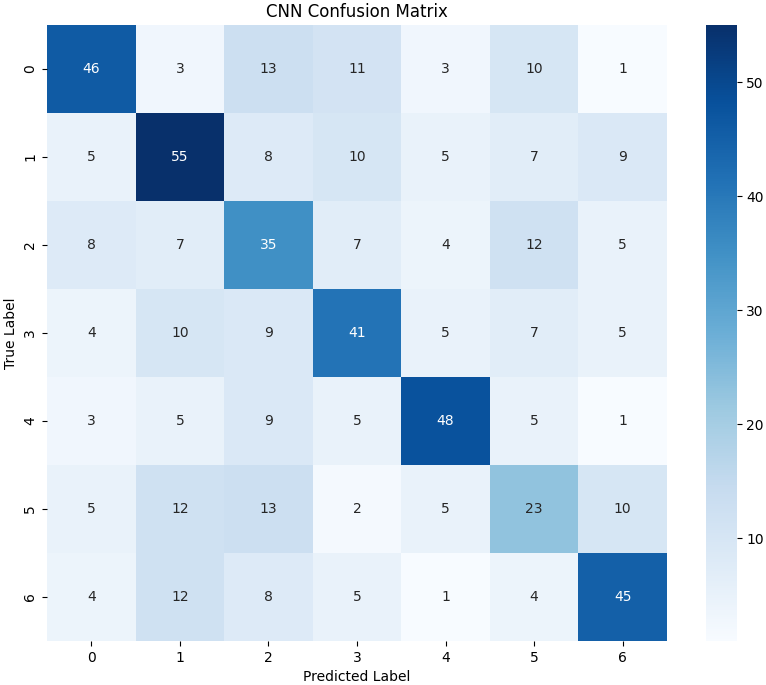
\includegraphics[width=\textwidth]{../image/confusion_matrix_final.png}
		\caption{AlexNet Confusion Matrix}
		\label{fig:confusion_matrix_alexnet}
	\end{minipage}
	\hfill
	\begin{minipage}{0.45\textwidth}
		\centering
		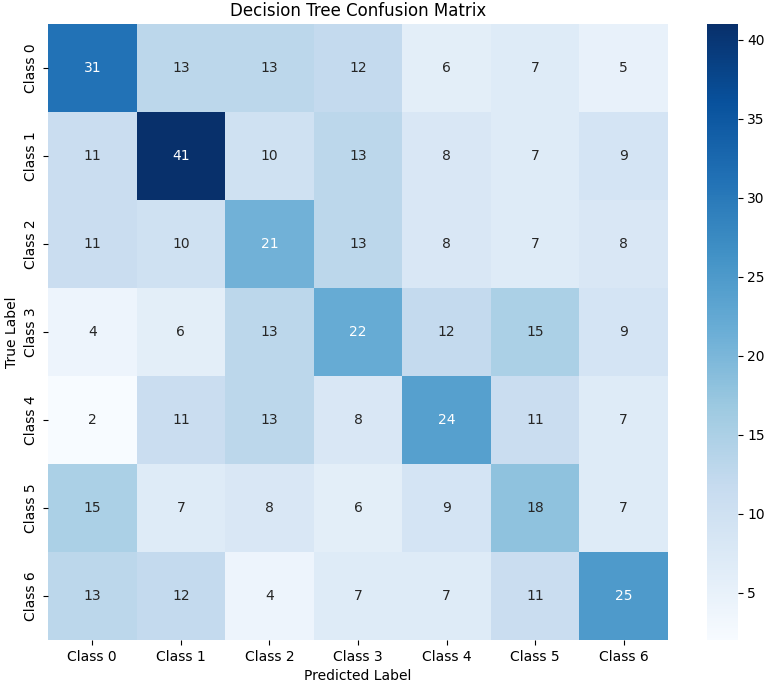
\includegraphics[width=\textwidth]{../../Lab4/image/confusion_matrix_decision_tree.png}
		\caption{Decision Tree Confusion Matrix}
		\label{fig:confusion_matrix_decision_tree}
	\end{minipage}
\end{figure}

\subsection{Other Performance Metrics}
\label{sec:other_performance_metrics}

We use accuracy, precision, recall, and F1 score as the performance metrics (which is embedded in a python library called \texttt{sklearn.metrics}). The comparison between the decision tree classifier and AlexNet is shown in Table~\ref{tab:performance_comparison}. The mathematical definitions of these metrics are shown in Appendix~\ref{app:performance_metrics}.

\begin{table}[ht]
	\centering
	\caption{Performance Comparison Between AlexNet and Decision Tree Classifier}
	\begin{tabular}{@{}lcccccccc@{}}
	\toprule
	\textbf{Class} & \textbf{Support} & \multicolumn{3}{c}{\textbf{AlexNet}} & \multicolumn{3}{c}{\textbf{Decision Tree}} \\ 
				   &                  & Precision & Recall & F1-Score       & Precision & Recall & F1-Score \\ \midrule
	Class 0 (paper)        & 87               & 0.61      & 0.53   & 0.57           & 0.3563    & 0.3563 & 0.3563   \\
	Class 1 (metal)        & 99               & 0.53      & 0.56   & 0.54           & 0.4100    & 0.4141 & 0.4121   \\
	Class 2 (plastic)        & 78               & 0.37      & 0.45   & 0.40           & 0.2561    & 0.2692 & 0.2625   \\
	Class 3 (glass)        & 81               & 0.51      & 0.51   & 0.51           & 0.2716    & 0.2716 & 0.2716   \\
	Class 4 (food)        & 76               & 0.68      & 0.63   & 0.65           & 0.3243    & 0.3158 & 0.3200   \\
	Class 5 (hazardous)       & 70               & 0.34      & 0.33   & 0.33           & 0.2368    & 0.2571 & 0.2466   \\
	Class 6 (electronic)       & 79               & 0.59      & 0.57   & 0.58           & 0.3571    & 0.3165 & 0.3356   \\ \midrule
	Accuracy       & 570              & \multicolumn{3}{c}{0.5140}          & \multicolumn{3}{c}{0.3193} \\ 
	Macro Avg      & 570              & 0.52      & 0.51   & 0.51           & 0.3160    & 0.3144 & 0.3149   \\ 
	Weighted Avg   & 570              & 0.52      & 0.51   & 0.52           & 0.3211    & 0.3193 & 0.3199   \\ \bottomrule
	\end{tabular}
	\label{tab:performance_comparison}
\end{table}

As shown in Table~\ref{tab:performance_comparison}, the AlexNet model outperforms the decision tree classifier in all metrics. The reason is still under research, but it is believed that decision tree classifier relies on manually extracted features (HOG), which are limited in capturing diverse and abstract patterns. On the other hand, AlexNet can automatically learn features from the data (using those convolutional kernels) and thus can capture more complex patterns. Also, the decision tree classifier is prone to overfitting, while for AlexNet, the dropout layer and batch normalization layer can prevent overfitting to some extent.

For a closer look at the performance of the two methods in each class, we find that for Class 2 (plastic) and Class 5 (hazardous), both methods have a low F1 score. This is probably because these two categories are even ambiguous to human, or share similar features with other classes. For example, hazardous waste can be also plastic, metal or electronic (which is often the case). Therefore, in the process of labeling, the human labeler may also confused about the class of the waste.

\section{Conclusion}

This project compares the Decision Tree Classifier and AlexNet in a multi-class image classification task. The evaluation results reveal that AlexNet significantly outperforms the Decision Tree Classifier across all performance metrics, achieving a test accuracy of $51.4\%$ compared to the Decision Tree’s $31.9\%$.

AlexNet’s superior performance can be attributed to its ability to automatically learn hierarchical and abstract features through convolutional layers, making it robust to complex image patterns. On the other hand, the Decision Tree’s reliance on manually extracted HOG features limits its capacity to generalize, leading to poorer performance.

Also from Section~\ref{sec:other_performance_metrics}, we learned that for a classifier, the classes should be well-defined and distinct, for a human classifier at least. Bad classification will result in badly-labelled dataset and thus a bad classifier. 

In conclusion, while Decision Trees may be suitable for simple classification tasks with well-defined features, deep learning models like AlexNet are more effective for complex, high-dimensional image data. Future work could explore hybrid approaches, combining handcrafted features and deep learning to improve classification performance further.

\newpage
\appendix
\section{Detailed AlexNet Architecture}
\label{app:alexnet}
\begin{table}[ht]
	\centering
	\caption{AlexNet Architecture}
	\begin{tabular}{@{}lll>{\raggedright\arraybackslash}p{3cm}@{}}
	\toprule
	\textbf{Layer Type}       & \textbf{Parameters}                 & \textbf{Input Size} & \textbf{Output Size} \\ \midrule
	Input                    & -                                  & $192\times192\times3$ & $192\times192\times3$ \\
	Conv2D + ReLU            & 64 filters, $11\times11$, stride 4 & $192\times192\times3$ & $48\times48\times64$  \\
	MaxPool2D                & $3\times3$, stride 2               & $48\times48\times64$  & $24\times24\times64$  \\
	Conv2D + ReLU            & 192 filters, $5\times5$            & $24\times24\times64$  & $24\times24\times192$ \\
	MaxPool2D                & $3\times3$, stride 2               & $24\times24\times192$ & $12\times12\times192$ \\
	Conv2D + ReLU            & 384 filters, $3\times3$            & $12\times12\times192$ & $12\times12\times384$ \\
	Conv2D + ReLU            & 256 filters, $3\times3$            & $12\times12\times384$ & $12\times12\times256$ \\
	Conv2D + ReLU            & 256 filters, $3\times3$            & $12\times12\times256$ & $12\times12\times256$ \\
	MaxPool2D                & $3\times3$, stride 2               & $12\times12\times256$ & $6\times6\times256$   \\
	AdaptiveAvgPool2D        & Output: $6\times6$                 & $6\times6\times256$   & $6\times6\times256$   \\
	Flatten                  & -                                  & $6\times6\times256$   & 9216                  \\
	Fully Connected (FC)     & 4096 neurons                       & 9216                  & 4096                  \\
	Fully Connected (FC)     & 4096 neurons                       & 4096                  & 4096                  \\
	Fully Connected (FC)     & 7 neurons (output)                 & 4096                  & 7                     \\ \bottomrule
	\end{tabular}
\end{table}

\section{Detailed Manual for All Codes}

\subsection{Training Set Splitting}
\label{app:splitting}

First, ensure you have the following directory structure:

% \lstinputlisting[language=bash, style=custombash]{folder-struct.txt} % bash


\begin{forest}
	for tree={
		font=\ttfamily,
		grow'=0,
		child anchor=west,
		parent anchor=south,
		anchor=west,
		calign=first,
		edge path={
			\noexpand\path [draw, \forestoption{edge}]
			(!u.south west) +(7.5pt,0) |- node[fill,inner sep=1.25pt] {} (.child anchor)\forestoption{edge label};
		},
		before typesetting nodes={
			if n=1
			{insert before={[,phantom]}}
			{}
		},
		fit=band,
		before computing xy={l=20pt},
	}
	[GUID\_FullName\_ML-Code/
		[mlenv/            \# Python environment]
		[Project2
			[2024\_uestc\_autlab/
				[data/
					[coco/ \# Original COCO dataset
						[JPEGImages/]
						[annotations.json]
					]
					[data\_coco\_test/annotations.json \# This will be generated
					]
					[data\_coco\_train/annotations.json \# This will be generated
					]
					[data\_coco\_valid/annotations.json \# This will be generated
					]
				]
				[split3.py]
				[train.py]
				[model.py]
				[dataset.py]
				[evaluate.py]
			]
			[image/
				[confusion\_matrix\_final.png]
			]
		]
		[Lab4/
			[coco/
				[annotations.json]
				[JPEGImages/]
			]
			[image/
				[confusion\_matrix\_decision\_tree.png]]
			[2024\_uestc\_autlab/
				[outputs/]
				[utils/]
				[dataset.py]
				[ml\_evaluate.py]
				[ml\_model.py]
			]
		]
	]
\end{forest}

In unix-like systems, you can run the following command to split the dataset:

% literal bash commands
\begin{lstlisting}[language=bash, style=custombash]
cd 2024_uestc_autlab
source mlenv/bin/activate
python split3.py
\end{lstlisting}

This will generate \texttt{data\_coco\_train}, \texttt{data\_coco\_valid}, and \texttt{data\_coco\_test} directories with the corresponding annotations.

\subsection{Image Preprocessing}

After correctly changing the directories, run:

\begin{lstlisting}[language=bash, style=custombash]
python dataset.py
\end{lstlisting}

The output will be:

\begin{lstlisting}[language=bash, style=custombash]
loading annotations into memory...
Done (t=0.01s)
creating index...
index created!
ID: 0, Label: paper
ID: 1, Label: metal
ID: 2, Label: plastic
ID: 3, Label: glass
ID: 4, Label: food
ID: 5, Label: hazardous
ID: 6, Label: electronic
2642
\end{lstlisting}

\subsection{Model Training}

Directly run:
% literal bash commands
\begin{lstlisting}[language=bash, style=custombash]
python train.py
\end{lstlisting}

About 30 epoches, the loss would be stable at around $0.2$, the accuracy would be roughly $0.5$.

\subsection{Performance Evaluation}

To evaluate the AlexNet model, run:
% literal bash commands
\begin{lstlisting}[language=bash, style=custombash]
python evaluate.py
\end{lstlisting}

This will print all the performance metrics and the figure of the confusion matrix under \texttt{./Project2/image/confusion\_matrix\_final.png}.


\section{Performace Metric Definitions}
\label{app:performance_metrics}

\subsection{Accuracy}

Accuracy measures the proportion of correctly classified instances out of the total instances. It is defined as:
$$
\text{Accuracy} = \frac{\text{Number of Correct Predictions}}{\text{Total Number of Predictions}}.
$$
For a confusion matrix:
$$
\text{Accuracy} = \frac{\sum_{i=1}^C \text{TP}_i}{\sum_{i=1}^C (\text{TP}_i + \text{FP}_i + \text{FN}_i)},
$$
where
\begin{itemize}
	\item $C$: Number of classes.
	\item $\text{TP}_i$: True Positives for class $i$.
	\item $\text{FP}_i$: False Positives for class $i$.
	\item $\text{FN}_i$: False Negatives for class $i$.
\end{itemize}


\subsection{Precision}

Precision measures the proportion of true positive predictions out of all predictions made for a particular class. It is defined as:
$$
\text{Precision}_i = \frac{\text{TP}_i}{\text{TP}_i + \text{FP}_i},
$$
where
\begin{itemize}
	\item $\text{TP}_i$: True Positives for class $i$.
	\item $\text{FP}_i$: False Positives for class $i$.
\end{itemize}

For multi-class classification, weighted average precision is:
$$
\text{Precision weighted avg} = \frac{\sum_{i=1}^C (\text{Precision}_i \cdot \text{Support}_i)}{\sum_{i=1}^C \text{Support}_i},
$$
where $\text{Support}_i$ is the number of true instances for class $i$.

\subsection{Recall}

Recall (or Sensitivity) measures the proportion of true positive predictions out of all actual instances for a particular class. It is defined as:
$$
\text{Recall}_i = \frac{\text{TP}_i}{\text{TP}_i + \text{FN}_i},
$$
where
\begin{itemize}
	\item $\text{TP}_i$: True Positives for class $i$.
	\item $\text{FN}_i$: False Negatives for class $i$.
\end{itemize}

For multi-class classification, weighted average recall is:
$$
\text{Recall weighted avg} = \frac{\sum_{i=1}^C (\text{Recall}_i \cdot \text{Support}_i)}{\sum_{i=1}^C \text{Support}_i}.
$$

\subsection{F1 Score}

The F1 Score is the harmonic mean of precision and recall, providing a balance between the two:
$$
\text{F1}_i = 2 \cdot \frac{\text{Precision}_i \cdot \text{Recall}_i}{\text{Precision}_i + \text{Recall}_i}.
$$
For multi-class classification, weighted average F1 score is:
$$
\text{F1 weighted avg} = \frac{\sum_{i=1}^C (\text{F1}_i \cdot \text{Support}_i)}{\sum_{i=1}^C \text{Support}_i}
$$

\subsection{Support}

For a class $c$ , the support is given by:
$$
\text{Support}_c = \sum_{i=1}^N \mathbf{1}(y_{\text{true},i} = c),
$$
where
\begin{itemize}
	\item $N$: Total number of samples in the dataset.
	\item $y_{\text{true},i}$: The true label for the $i$-th sample.
	\item $\mathbf{1}(\text{condition})$: Indicator function that equals 1 if the condition is true, and 0 otherwise.
\end{itemize}

\newpage
\section{All Related Python Code}

\subsection{\texttt{dataset.py}}
\label{app:dataset_py}

\lstinputlisting[caption={Experiment Code for Image Preprocessing}, label={lst:dataset_py}, language=Python, style=custompython]{../2024_uestc_autlab/dataset.py} % python

\subsection{\texttt{model.py}}
\label{app:model_py}

\lstinputlisting[caption={AlexNet Structure}, label={lst:model_py}, language=Python, style=custompython]{../2024_uestc_autlab/model.py} % python

\subsection{\texttt{train.py}}
\label{app:train_py}

\lstinputlisting[caption={Training Code}, label={lst:train_py}, language=Python, style=custompython]{../2024_uestc_autlab/train.py} % python

\subsection{\texttt{evaluate.py}}
\label{app:evaluate_py}

\lstinputlisting[caption={Evaluation Code}, label={lst:evaluate_py}, language=Python, style=custompython]{../2024_uestc_autlab/evaluate.py} % python


% \addcontentsline{toc}{section}{References}
% \bibliographystyle{plain} % We choose the "plain" reference style
% \bibliography{General} % Entries are in the refs.bib file

\end{document}

